\documentclass[12pt]{article}

\usepackage{sbc-template}
\usepackage{graphicx,url}
\usepackage[brazil]{babel}   
\usepackage[utf8]{inputenc}  

\sloppy

\title{IncluiDev: Desenvolvimento e Avaliação de uma Plataforma Baseada em Evidências para Apoio ao Ensino de Programação para Pessoas com Deficiência Visual}

\author{Lucas R. Pedro\inst{1}, Esteice Janaina Santos Batista\inst{1}}

\address{Faculdade de Computação -- Universidade Federal de Mato Grosso do Sul (UFMS)\\
  Campo Grande -- MS -- Brazil
  \email{lucas.pedro@ufms.br, esteic.batista@ufms.br} 
}

\begin{document} 

\maketitle

\begin{abstract}
  The inclusion of blind and visually impaired (BVI) individuals in Computer Science presents significant challenges due to the historical dependence on visual metaphors in programming languages and environments \cite{stefik2013empirical}. Although studies, tools, and guidelines for accessible programming education exist, these resources are highly fragmented across literature and the web. This study aims to develop and evaluate a centralized repository, named \textit{IncluiDev}, which organizes and provides these tools, methods, and scientific papers. The repository was built as an accessible web application and features a ``Guided Assistant'', a dynamic recommendation system based on user profiles (Students, Teachers, Developers, and Researchers). Accessibility compliance was validated through automated audits (Google Lighthouse, WAVE) and manual testing with screen readers and keyboard navigation. As a preliminary heuristic step, the recommendation logic was also assessed through LLM-simulated user personas applying the System Usability Scale (SUS) \cite{brooke1996sus} and the Technology Acceptance Model (TAM) \cite{davis1989tam}; empirical validation with real participants is planned as future work.
\end{abstract}
     
\begin{resumo} 
  A inclusão de Pessoas com Deficiência Visual (PcDV) no campo da Ciência da Computação apresenta desafios significativos devido à histórica dependência de metáforas visuais em linguagens e ambientes de programação \cite{stefik2013empirical}. Apesar da existência de estudos, ferramentas e diretrizes voltadas para a acessibilidade no ensino de programação, esses recursos encontram-se dispersos na literatura e na web. O objetivo deste estudo é desenvolver e avaliar um repositório centralizado, denominado \textit{IncluiDev}, que organiza e disponibiliza essas ferramentas, métodos e artigos científicos. O repositório foi construído como uma aplicação web acessível e incorpora um ``Assistente Guiado'', um sistema de recomendação dinâmico baseado em perfis de usuário (Estudantes, Professores, Desenvolvedores e Pesquisadores). A conformidade de acessibilidade foi validada por meio de auditorias automatizadas (Google Lighthouse, WAVE) e testes manuais com leitores de tela e navegação por teclado. Como etapa preliminar e heurística, a lógica de recomendação também foi avaliada por meio de personas simuladas por agentes de IA, aplicando as escalas SUS \cite{brooke1996sus} e TAM \cite{davis1989tam}; a validação empírica com participantes reais está prevista como trabalho futuro.
\end{resumo}

\section{Introdução}

A inclusão digital de Pessoas com Deficiência Visual (PcDV) nas áreas de Ciência da Computação e Tecnologia da Informação (TI) tem se mostrado cada vez mais essencial em uma sociedade fortemente impulsionada pela tecnologia. O ensino de programação tradicionalmente exige a compreensão de metáforas visuais complexas, como diagramas de fluxo, código em blocos coloridos e a própria indentação textual \cite{resnick2009scratch}, criando barreiras significativas de aprendizagem para estudantes cegos ou com baixa visão.

A comunidade acadêmica e de desenvolvimento tem respondido a essas barreiras por meio da criação de linguagens baseadas em evidências, como a Quorum Language \cite{stefik2019quorum}, ambientes tangíveis como o Code Jumper \cite{morrison2019physical}, e a adaptação de leitores de tela em IDEs de mercado \cite{seo2023coding}. No entanto, o desenvolvimento dessas soluções, por si só, não garante o acesso ao usuário final.

\subsection{Problema de Pesquisa}
Apesar do crescente número de estudos sobre o ensino de programação para PcDV, os recursos encontram-se dispersos, dificultando sua localização e utilização prática por diferentes públicos. Professores em busca de metodologias de ensino, desenvolvedores buscando diretrizes de acessibilidade e os próprios estudantes enfrentam a tarefa de buscar soluções fragmentadas em diversas fontes. Diante desse cenário, este trabalho busca responder à seguinte questão de pesquisa: como centralizar, classificar e recomendar de forma acessível metodologias, ferramentas e pesquisas sobre o ensino de programação para PcDV?

\subsection{Objetivos}
O objetivo geral deste trabalho é construir e avaliar um portal web dinâmico e centralizado que funcione como um repositório interativo de práticas, ferramentas e estudos voltados ao ensino de programação para PcDV.

Para alcançar este propósito, foram definidos os seguintes objetivos específicos:
\begin{itemize}
    \item Organizar os recursos identificados na literatura acadêmica e na indústria em uma taxonomia coerente;
    \item Desenvolver um repositório web que respeite as diretrizes de acessibilidade WCAG 2.1 nível AA \cite{wcag21};
    \item Implementar um sistema de recomendações (``Assistente Guiado'') baseado em jornadas de perfis (Estudante, Professor, Pesquisador e Desenvolvedor);
    \item Avaliar a usabilidade, a aceitação e a acessibilidade do sistema utilizando métodos empíricos e escalas padronizadas \cite{brooke1996sus, davis1989tam}.
\end{itemize}

\subsection{Organização do artigo}
O restante deste artigo está organizado da seguinte forma: a Seção 2 apresenta o Referencial Teórico sobre o ensino acessível e os métodos de avaliação. A Seção 3 detalha os Métodos aplicados na construção do repositório e os procedimentos de validação. A Seção 4 reporta os Resultados alcançados, enquanto a Seção 5 discute as implicações desses achados. Finalmente, a Seção 6 traz a Conclusão e os trabalhos futuros.

\section{Referencial Teórico} \label{sec:referencial}

\subsection{Ensino de Programação para Pessoas com Deficiência Visual}
A compreensão de lógicas algorítmicas por indivíduos videntes frequentemente se apoia em recursos visuais como diagramas de bloco, pseudocódigos formatados e interfaces baseadas em interações de arrastar e soltar, a exemplo do Scratch \cite{resnick2009scratch}. Para PcDV, a dependência quase exclusiva desses artefatos representa uma barreira significativa para o ensino e a prática de programação \cite{hadwen2018making}.

Estudos na área apontam que a principal dificuldade reside na sobrecarga cognitiva imposta pela leitura sequencial dos leitores de tela \cite{baker2015structjumper}. Um programador vidente visualiza a estrutura de um laço de repetição ou de uma estrutura condicional de forma global por meio da indentação espacial. Em contrapartida, um usuário de leitor de tela necessita memorizar a estrutura lógica enquanto escuta o código linha por linha \cite{baker2019educational}.

Para mitigar tais desafios, diferentes estratégias educacionais e tecnologias assistivas têm sido propostas. Abordagens baseadas em áudio e sonificação de código --- onde blocos e erros emitem sons característicos em um ambiente acústico --- e ambientes tangíveis, como a programação física utilizando hardwares modulares conectáveis \cite{codejumper2019}, são exemplos de intervenções com eficácia demonstrada no ensino inclusivo \cite{stefik2013empirical}.

\subsection{Recursos e Tecnologias para Inclusão}
Duas estratégias distintas emergem na literatura: a adaptação de ferramentas já consolidadas e o desenvolvimento de novos ambientes e linguagens projetados desde a origem para acessibilidade. Ferramentas consolidadas no mercado, como o Visual Studio Code, implementaram modos de acessibilidade e atalhos otimizados, facilitando a navegação com leitores de tela \cite{seo2023coding, vscode_accessibility}. Paralelamente, linguagens de programação concebidas sob a perspectiva de evidências de usabilidade, como a linguagem Quorum \cite{stefik2019quorum}, contribuíram para reduzir a dependência de caracteres especiais complexos, otimizando a leitura fonética realizada por softwares de síntese de voz.

Apesar da crescente disponibilidade tecnológica, a aplicabilidade efetiva dessas ferramentas depende da curadoria da informação e do acesso a guias e diretrizes atualizadas, como as Diretrizes de Acessibilidade para Conteúdo Web (WCAG) \cite{wcag21}. A organização sistemática desses materiais em repositórios qualificados é essencial para que os educadores não precisem criar adaptações pedagógicas a partir do zero, promovendo o reuso e a padronização das intervenções de acessibilidade digital.

\subsection{Avaliação de Sistemas Educacionais}
A validação de portais e repositórios educacionais exige o uso de instrumentos confiáveis de avaliação. A \textit{System Usability Scale} (SUS) \cite{brooke1996sus} é um questionário de dez itens, padronizado internacionalmente, amplamente adotado para medir de forma rápida e quantitativa a usabilidade global de uma interface tecnológica.

De maneira complementar, o \textit{Technology Acceptance Model} (TAM) \cite{davis1989tam} é utilizado para avaliar a utilidade percebida e a facilidade de uso percebida, fatores que determinam a intenção comportamental e a adoção do sistema pelo usuário.

No contexto da acessibilidade digital, esses modelos quantitativos, quando complementados por questões qualitativas abertas, fornecem um conjunto robusto de evidências sobre as barreiras enfrentadas durante a interação e o nível de satisfação do usuário.

\section{Método}

A presente pesquisa caracteriza-se como um estudo de natureza aplicada, conduzido sob uma abordagem de métodos mistos (quantitativa e qualitativa). O escopo do desenvolvimento foi estruturado com base nos achados de uma Revisão de Literatura preliminar, a qual identificou e catalogou diretrizes metodológicas, ferramentas de software, aplicações lúdicas educacionais e estudos empíricos centrados na interseção entre o ensino de programação e a deficiência visual.

\subsection{Desenvolvimento do Repositório}
O repositório digital, nomeado \textit{IncluiDev}, foi projetado segundo a arquitetura de \textit{Single Page Application} (SPA), utilizando a biblioteca React \cite{react2023} juntamente com o empacotador Vite \cite{vite2023} e o ambiente Node.js. A versão de produção da plataforma pode ser acessada através do endereço \url{https://incluidev-portal.vercel.app/}.

A concepção arquitetural priorizou o desenvolvimento de componentes funcionais acessíveis, garantindo a incorporação nativa de atributos WAI-ARIA \cite{waiaria12}, como as propriedades \textit{aria-live} para atualizações dinâmicas e \textit{aria-labelledby} para estruturação semântica.

O processo contínuo de catalogação do estado da arte gerou uma taxonomia bidimensional, na qual cada recurso levantado é mapeado e indexado em função do Nível de Ensino (Básico, Técnico, Superior) e do Público-Alvo primário.

As permissões, os papéis e a estrutura de interações dos diferentes perfis com as ferramentas disponíveis na aplicação encontram-se representados no Diagrama de Casos de Uso (Figura~\ref{fig:casosdeuso}).

\begin{figure}[htpb]
  \centering
  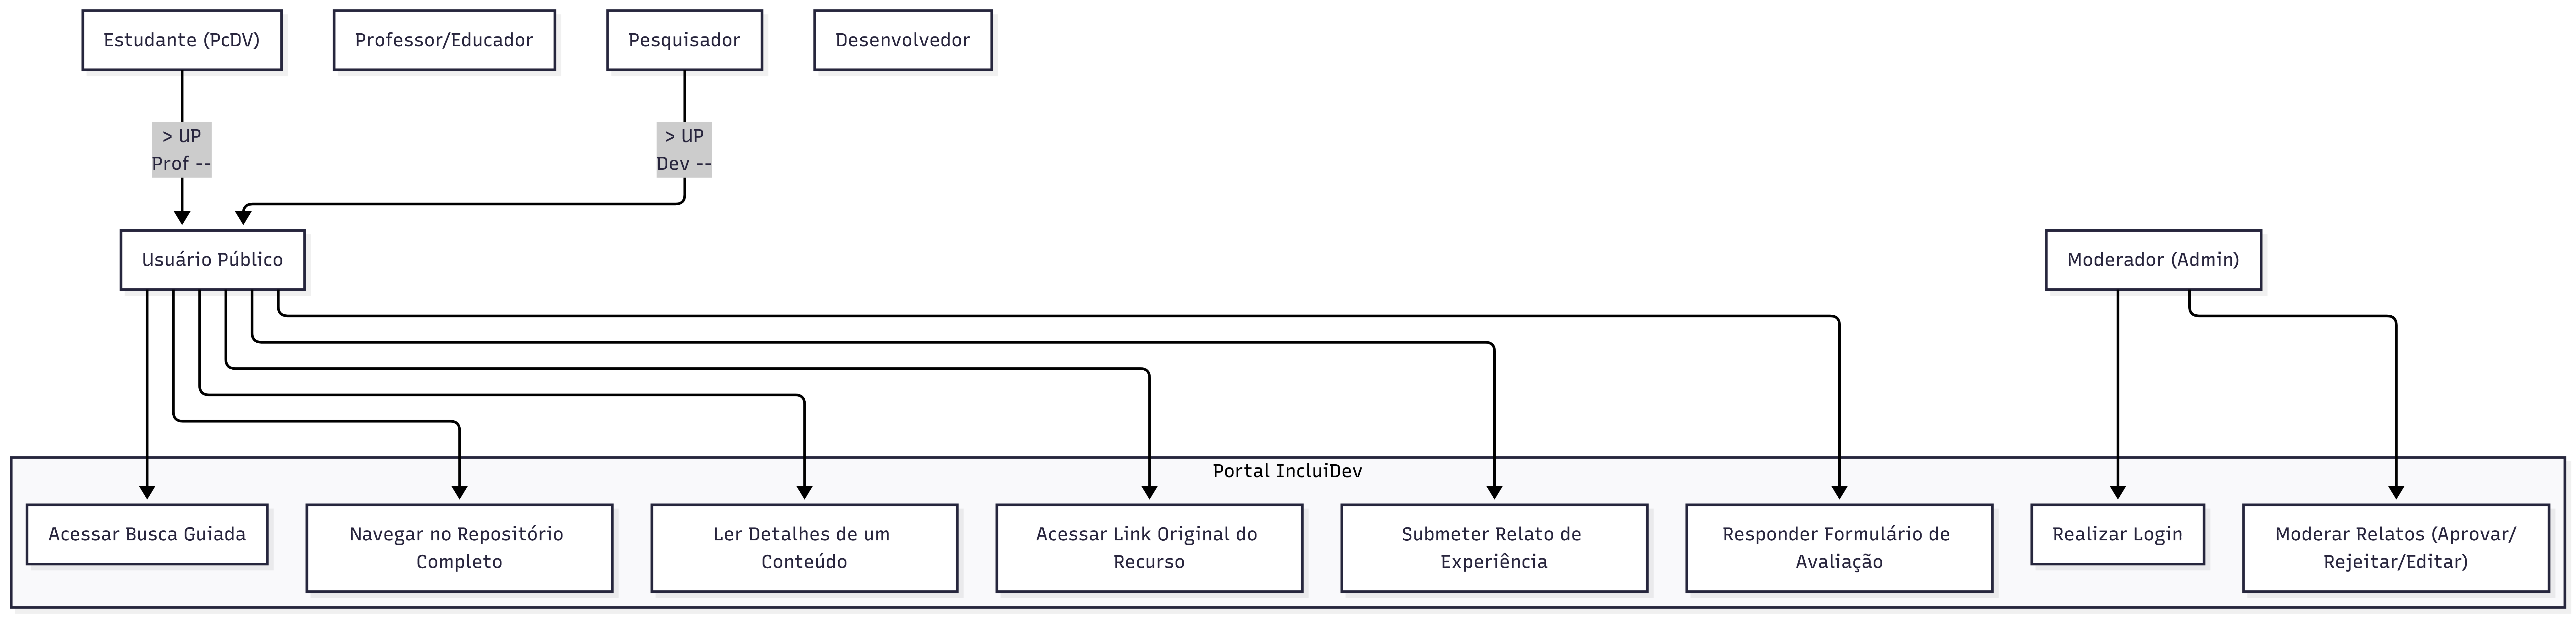
\includegraphics[width=0.8\textwidth]{diagrama_casos_de_uso.png}
  \caption{Diagrama de Casos de Uso do Portal IncluiDev}
  \label{fig:casosdeuso}
\end{figure}

\subsection{Construção do Assistente Guiado}
Para superar as limitações dos mecanismos tradicionais de filtragem e pesquisa em tabela, foi proposto o ``Assistente Guiado'': um sistema de recomendação guiado por perfil de usuário.

Diferentemente de uma listagem estática de filtros, o sistema orienta o usuário a uma autoidentificação com base em quatro perfis identificados na literatura: Estudante, Professor, Desenvolvedor e Pesquisador.

A partir do perfil selecionado, a aplicação apresenta perguntas de múltipla escolha focadas no objetivo pedagógico ou técnico principal (por exemplo, exploração de ferramentas baseadas em áudio ou obtenção de referências de revisões sistemáticas). O sistema compara as respostas do usuário com as \textit{tags} dos conteúdos cadastrados, apresentando recomendações relevantes sem sobrecarregar o usuário de tecnologias assistivas.

O fluxo percorrido pelo usuário, desde a seleção de perfil até a exibição dos resultados pelo sistema de recomendação, está ilustrado na Figura~\ref{fig:fluxograma}.

\begin{figure}[htpb]
  \centering
  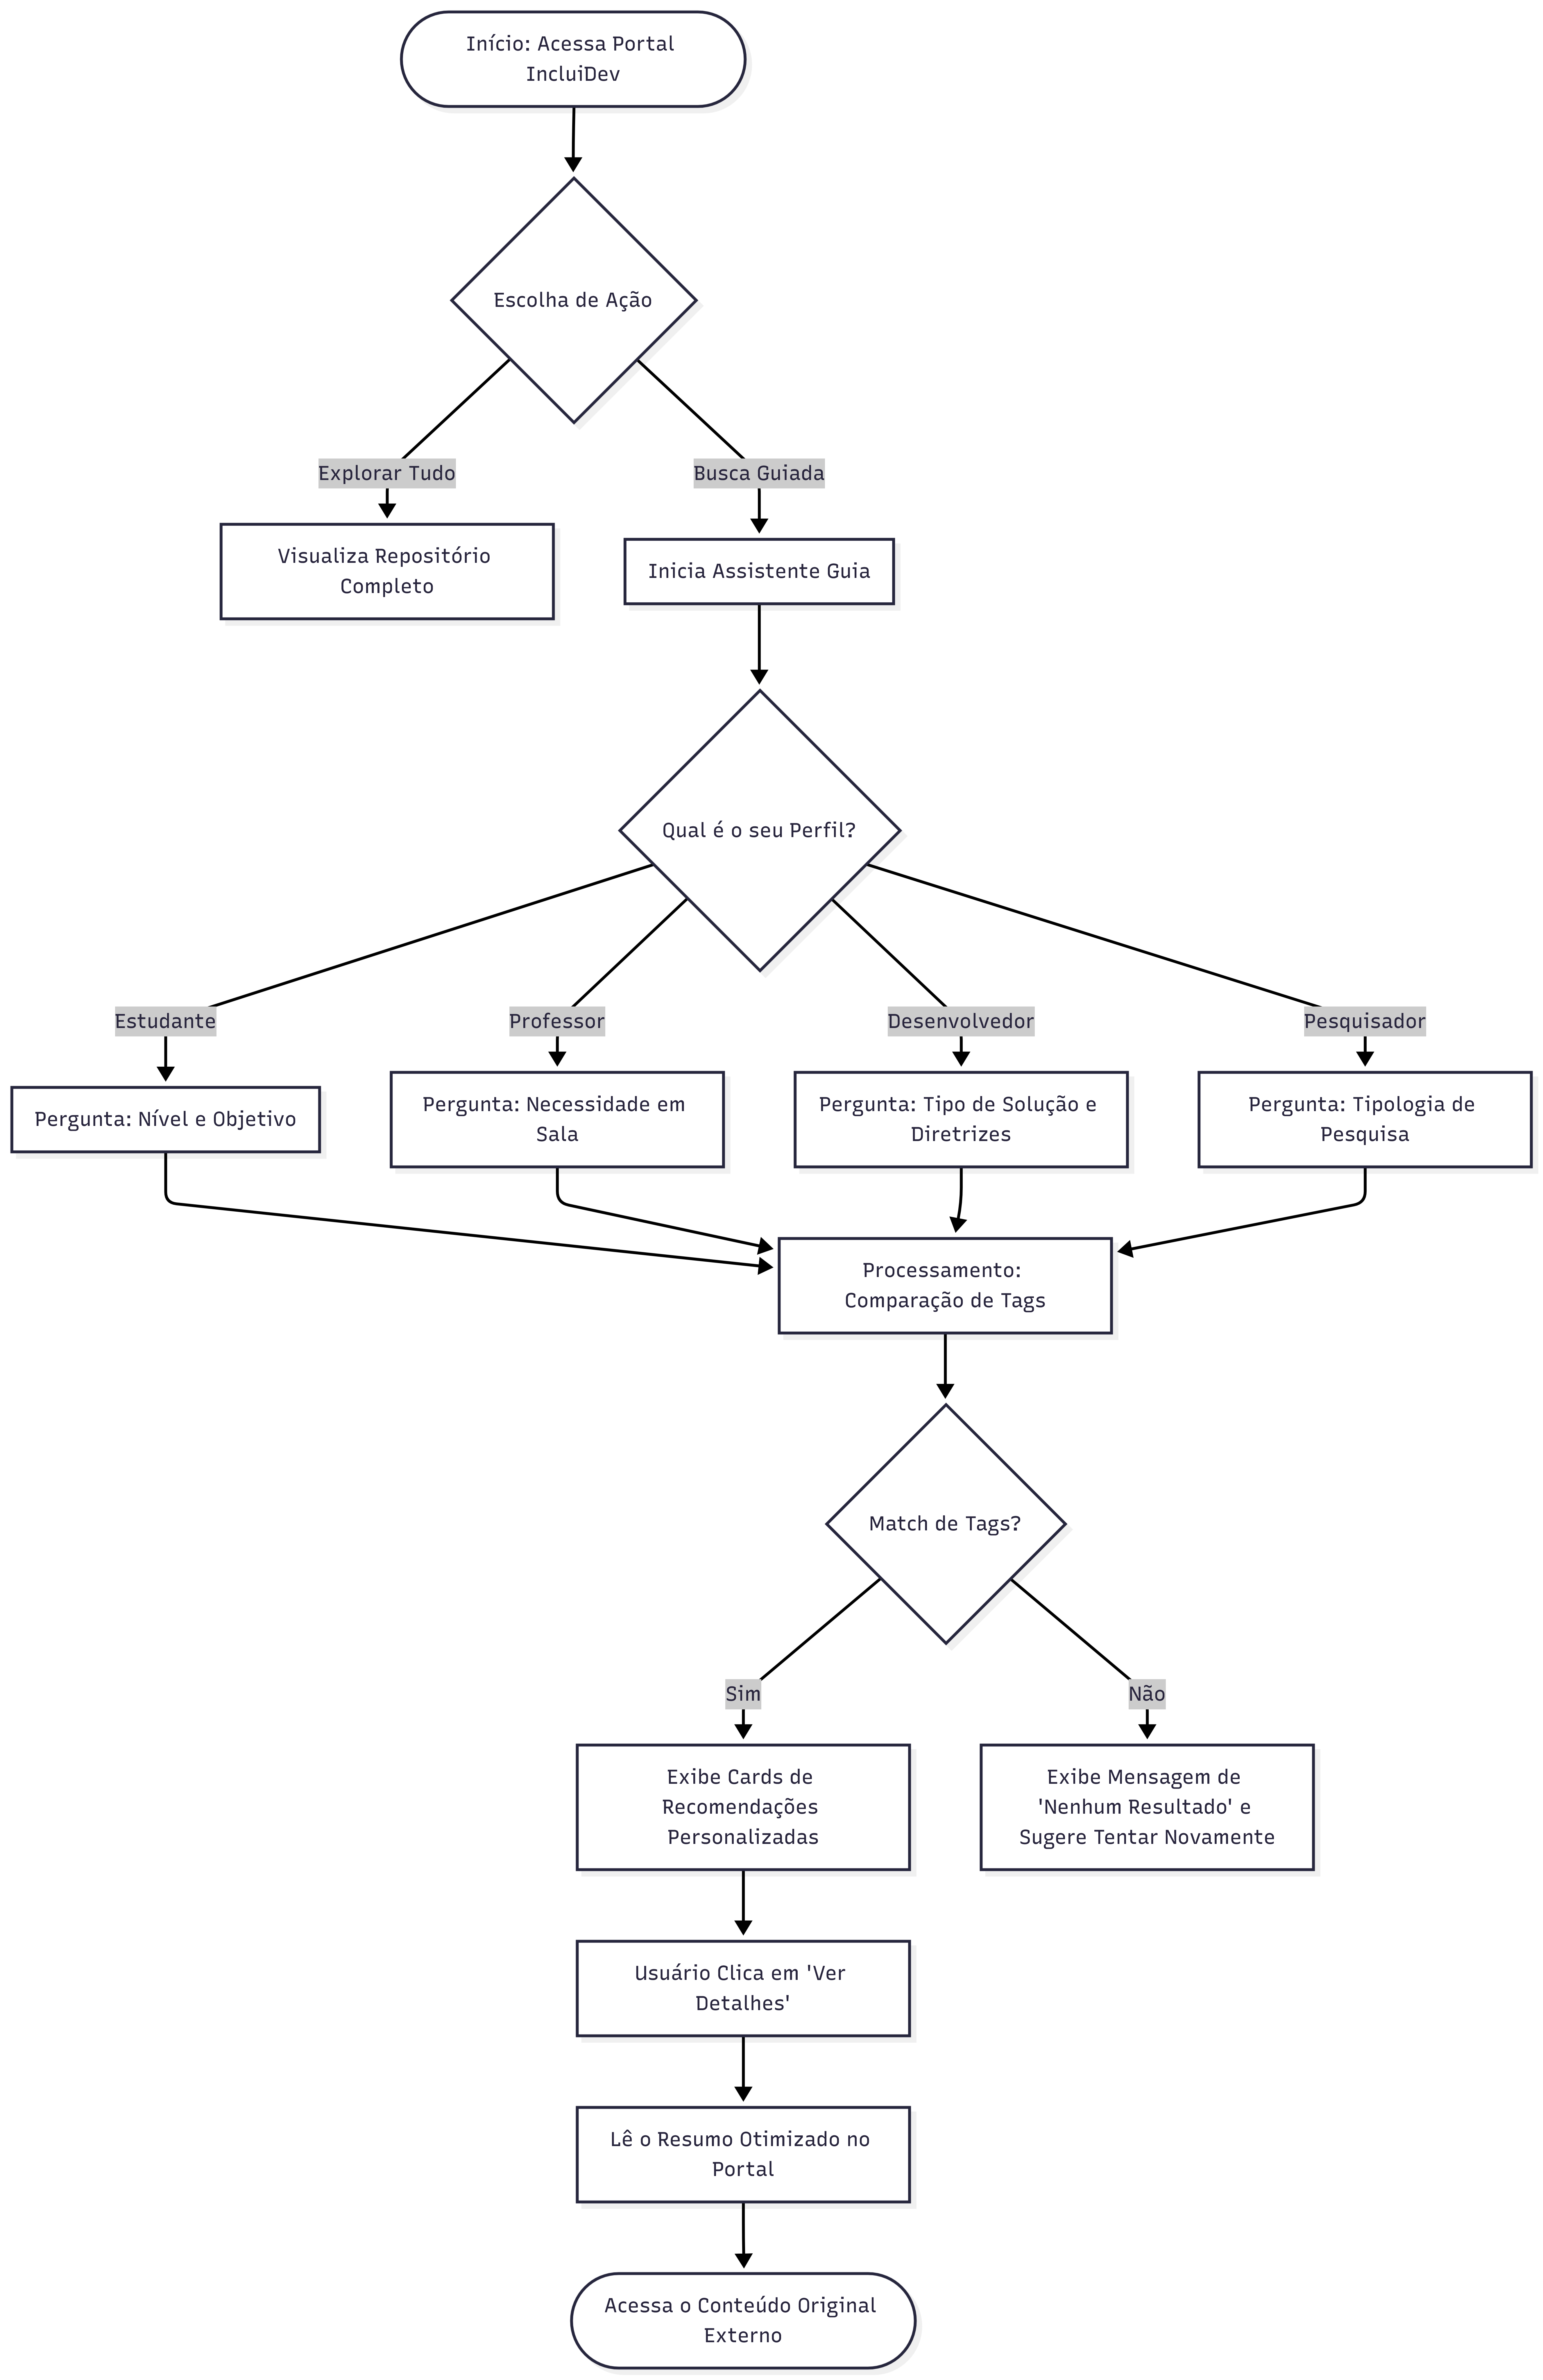
\includegraphics[width=1\textwidth]{fluxograma_navegacao.png}
  \caption{Fluxograma de Navegação do Assistente Guiado}
  \label{fig:fluxograma}
\end{figure}

\subsection{Avaliação do Sistema}
O protocolo de validação do repositório foi estruturado em fases. Como etapa preliminar para homologação da arquitetura lógica do sistema, empregou-se a simulação por Agentes de IA (LLMs) como avaliadores heurísticos, técnica fundamentada na literatura recente sobre simulação de usuários em avaliações de interação humano-computador \cite{seshadri2026lost}. O mesmo estudo alerta que agentes de IA constituem \textit{proxies} não confiáveis para usuários humanos reais, apresentando descalibração de julgamento e ausência de fadiga sensorial genuína; por esse motivo, os resultados desta etapa são tratados aqui como indicadores heurísticos preliminares, e não como medidas psicométricas validadas.

Os agentes foram instruídos a interpretar os quatro perfis de usuário mapeados (Estudante, Professor, Pesquisador e Desenvolvedor), interagindo com a plataforma e respondendo, em formato dissertativo, aos itens da \textit{System Usability Scale} (SUS) \cite{brooke1996sus} e do \textit{Technology Acceptance Model} (TAM) \cite{davis1989tam}. Esta simulação funciona como uma validação heurística preparatória, garantindo a coesão lógica e a acessibilidade técnica da aplicação antes da condução de testes empíricos com grupos representativos de participantes reais, prevista como próxima etapa do projeto.

\section{Resultados}

\subsection{Caracterização do Repositório}
A etapa de curadoria e extração consolidou um catálogo contendo 34 recursos fundamentais, classificados segundo a taxonomia proposta. A categorização buscou ser abrangente, incluindo tanto \textit{frameworks} de alcance global (como as diretrizes de acessibilidade W3C \cite{wcag21} e a documentação MDN \cite{mdn2024}) quanto ambientes lúdicos e tangíveis focados na iniciação do pensamento computacional sem monitor, como o Code Jumper \cite{morrison2019physical} e linguagens baseadas em evidências como a Quorum \cite{stefik2019quorum}.

O portal oferece interfaces que reúnem resumos detalhados com acesso direcionado às fontes científicas originais, para que professores e desenvolvedores encontrem referências técnicas e legais em um único lugar.

O código-fonte completo do sistema, bem como os artefatos de validação descritos nas seções seguintes, estão disponíveis no repositório público do projeto: \url{https://github.com/lucasmantovany/incluidev-portal}.

Para ilustrar a interface da aplicação, a Figura~\ref{fig:print_home} apresenta a tela inicial do portal, destacando o acesso rápido por perfis e níveis de ensino. A Figura~\ref{fig:print_repositorio} demonstra a tela do repositório com o Assistente Guiado e a listagem de recursos.

\begin{figure}[htpb]
  \centering
  \includegraphics[width=1\textwidth]{print_home.png}
  \caption{Tela Inicial do Portal IncluiDev}
  \label{fig:print_home}
\end{figure}

\begin{figure}[htpb]
  \centering
  \includegraphics[width=1\textwidth]{print_repositorio.png}
  \caption{Tela do Repositório e Filtros do Assistente}
  \label{fig:print_repositorio}
\end{figure}

\subsection{Funcionamento do Assistente Guiado}
A implementação do Assistente Guiado confirmou, durante os testes técnicos, que as árvores de decisão e o sistema de cruzamento de \textit{tags} retornam ao menos uma recomendação em todos os cenários cobertos pelo acervo atual. O fluxo responsivo adaptou-se de forma consistente às variações de contexto para cada um dos quatro perfis, mantendo a compatibilidade com leitores de tela nos ambientes de teste.

O arranjo visual limpo, sem \textit{pop-ups} inesperados, facilita a navegação independente por usuários que dependem de interações exclusivamente via teclado.

\subsection{Avaliação de Acessibilidade}
Para avaliar o cumprimento das diretrizes de acessibilidade WCAG 2.1 (Nível AA), foram realizadas auditorias mistas. A avaliação automatizada com o Google Lighthouse apontou alta conformidade, e a ferramenta WAVE confirmou a ausência de erros estruturais, indicando apenas alertas pontuais de contraste de cores em elementos secundários. A síntese dos escores obtidos é apresentada na Tabela~\ref{tab:acessibilidade}.

\begin{table}[htpb]
  \centering
  \caption{Resultados das auditorias automatizadas de acessibilidade}
  \label{tab:acessibilidade}
  \begin{tabular}{lcc}
    \hline
    \textbf{Ferramenta / Métrica} & \textbf{Desktop} & \textbf{Móvel} \\
    \hline
    Google Lighthouse (escore de Acessibilidade) & 96/100 & 95/100 \\
    WAVE -- Erros estruturais & 0 & 0 \\
    WAVE -- Alertas de contraste (elementos secundários) & Pontuais & Pontuais \\
    \hline
  \end{tabular}
\end{table}

Cabe ressaltar uma limitação importante deste processo: ferramentas automatizadas são capazes de detectar, em média, apenas cerca de 40\% dos erros de acessibilidade em uma interface web. Por esta razão, a auditoria manual, conduzida individualmente pelo pesquisador utilizando leitores de tela e navegação estrita por teclado, desempenhou papel fundamental.

Na auditoria manual, verificou-se o funcionamento adequado da navegação por teclado, sem a ocorrência de armadilhas de foco (\textit{keyboard traps}). Além disso, a aplicação utiliza regiões dinâmicas (\texttt{aria-live="assertive"}) de forma correta, garantindo que as mudanças de tela do Assistente Guiado sejam lidas imediatamente por leitores de tela como o NVDA, o que evita a desorientação do usuário.

\subsection{Validação Simulatória por Agentes de IA}
Como etapa preliminar de validação estrutural e lógica da interface, a avaliação de usabilidade foi conduzida utilizando a simulação por Agentes de IA (\textit{LLM-Simulated Users}), uma abordagem apoiada por estudos recentes na área de interação humano-computador. Esta etapa inicial visa assegurar a coesão do fluxo de navegação antes de submeter a plataforma a testes empíricos com usuários reais. Para isso, foram elaborados \textit{prompts} de sistema simulando as quatro personas do projeto: Estudante, Professor, Pesquisador e Desenvolvedor. O registro completo desse processo --- os \textit{prompts} utilizados e as respostas geradas pelos quatro agentes --- está disponível para consulta no repositório público do projeto, garantindo a transparência metodológica desta etapa.

A interação simulada das quatro personas com o Assistente Guiado resultou em respostas consistentemente favoráveis aos itens do SUS e do TAM, sem que nenhuma das personas reportasse obstáculos estruturais de navegação ou de compreensão do fluxo. As justificativas dissertativas geradas pelos agentes apontaram, de forma qualitativa, baixa carga percebida de leitura sequencial e alta utilidade percebida na recomendação direcionada por perfil --- a persona de Estudante, por exemplo, registrou: \textit{``A interface fez perguntas objetivas. Não tive que ler centenas de links de pesquisa, o que aliviou minha fadiga com o NVDA''} --- e a persona de Pesquisador comparou favoravelmente a busca guiada a consultas booleanas tradicionais.

Uma análise temática das quatro respostas revela um padrão recorrente entre os perfis de Estudante, Professor e Pesquisador: todos destacaram a redução do esforço de busca e leitura sequencial como o principal benefício percebido, contrastando a experiência guiada com a navegação tradicional por mecanismos de busca genéricos ou bases bibliográficas extensas. Já a persona de Desenvolvedor enfatizou um eixo distinto, voltado à completude técnica e à ausência de ruído informacional na apresentação dos recursos. Essa diferença sugere que, embora o Assistente Guiado atenda de forma consistente à necessidade central de reduzir a sobrecarga de navegação, futuras iterações do sistema poderiam explorar critérios de relevância específicos por perfil --- por exemplo, priorizando profundidade técnica para Desenvolvedores e amplitude de fontes para Pesquisadores. Tais padrões, contudo, derivam de uma simulação textual e devem ser interpretados como hipóteses a confirmar com usuários reais, e não como conclusões definitivas sobre o comportamento do público-alvo.

É importante destacar que esses resultados não substituem uma medição psicométrica real: por se tratar de uma simulação textual, os valores eventualmente atribuídos pelos agentes às escalas SUS e TAM não possuem o mesmo lastro de validade que escores coletados com usuários humanos. Eles são reportados aqui apenas como sinalização heurística de que a arquitetura lógica do sistema não apresenta inconsistências graves nos quatro fluxos avaliados, servindo de base para a etapa de validação empírica planejada como trabalho futuro (Seção 6).

\section{Discussão}
Os resultados obtidos nos testes de acessibilidade e nas simulações de usabilidade indicam que a estrutura do \textit{IncluiDev} atende de forma satisfatória aos requisitos técnicos e práticos propostos para esta primeira fase do projeto. Os altos escores nas avaliações sugerem que a busca orientada por perfis facilita o acesso à informação e reduz o esforço necessário na navegação. A etapa atual de validação com Agentes de IA atua como um filtro rigoroso de qualidade, consolidando a base lógica do portal. É importante ressaltar que esta metodologia não substitui a experiência humana, uma vez que Modelos de Linguagem tendem a gerar avaliações otimistas e não vivenciam barreiras sensoriais orgânicas. Contudo, os resultados atestam a viabilidade tecnológica da ferramenta desenvolvida, estabelecendo uma fundação sólida para que futuras iterações da pesquisa contemplem a validação empírica direta com o público-alvo.

\section{Conclusão}
A inclusão de Pessoas com Deficiência Visual no ensino de programação é um desafio complexo, historicamente agravado pela dispersão de ferramentas e metodologias acessíveis. Este estudo apresentou o \textit{IncluiDev}, um repositório centralizado e dinâmico, projetado para mitigar essa fragmentação por meio de uma taxonomia estruturada e de uma navegação orientada a perfis de usuário.

Os resultados das auditorias técnicas atestaram que a ferramenta atinge altos padrões de acessibilidade, cumprindo rigorosamente as diretrizes da WCAG 2.1. Adicionalmente, a etapa preliminar de validação lógica, conduzida por meio da simulação com Agentes de IA, indicou que o ``Assistente Guiado'' apresenta excelente usabilidade e eficácia em recomendar soluções precisas para Estudantes, Professores, Pesquisadores e Desenvolvedores. A arquitetura proposta mostrou-se capaz de reduzir a carga cognitiva exigida durante a navegação via leitores de tela.

Como discutido na Seção 5, as principais limitações deste estudo decorrem da natureza preliminar da validação por agentes de IA --- que não substitui a experiência de usuários reais --- e da ausência de testes empíricos com participantes humanos, motivada pelo prazo hábil da pesquisa para submissão. Soma-se a isso o fato de que ferramentas automatizadas de acessibilidade, como discutido na Seção 4.3, capturam apenas uma fração dos problemas reais de interação da interface. Por isso, como trabalhos futuros, torna-se essencial a execução de testes empíricos com grupos representativos de participantes, em especial pessoas com deficiência visual --- tanto discentes quanto docentes desse público, que poderão utilizar o sistema com frequência ---, bem como a comparação dos resultados simulados de SUS/TAM com avaliações conduzidas com usuários reais.

Espera-se que o portal \textit{IncluiDev} gere um impacto positivo imediato ao facilitar o encontro de ferramentas e metodologias de programação inclusiva, reduzindo o tempo de pesquisa de educadores e estudantes. Com isso, o projeto busca contribuir para a pesquisa tecnológica educacional e para o fomento de um ensino de computação mais inclusivo e estruturado. Adicionalmente, a expansão contínua da base de dados catalogada e o aprimoramento das heurísticas de recomendação constituem os próximos passos para consolidar o IncluiDev como ferramenta de referência nesse ecossistema.

\bibliographystyle{sbc}
\bibliography{references}

\end{document}
